%\documentclass[12pt,onecolumn,letterpaper]{article}
\documentclass[12pt]{article}
\usepackage[cmex10]{amsmath}
\usepackage{algorithmic}
\usepackage{array}
\usepackage{color}
\usepackage{graphicx}
\usepackage{caption}
\usepackage{subcaption}
\usepackage{listings}
\usepackage{float}
\usepackage{subfiles} % For my use of typesetable work files
\usepackage{flushend} % Used for creating equal length columns at the end
\usepackage{paralist} % Used for allowing in paragraph lists.
\usepackage{setspace}
\usepackage{fancyhdr}
\usepackage{lastpage}
\usepackage{hyperref}
\usepackage{xcolor}
\usepackage{lipsum}
\usepackage{enumitem}
\usepackage{rotating}
\usepackage[margin=0.75in, bottom=1in, top=0.25in, includeheadfoot]{geometry}

\renewcommand{\headrulewidth}{1pt}
\pagenumbering{gobble}
\begin{document}
%%----Setup Document Data----
\def \doctitle {Active HF Dipole Balun} %Main Title
\def \docsubtitle {Initial Design Document} %Sub Title, document type?
\def \docid	 {AHFDB-IDD}  %%Document ID, should be shorthand
\def \docvers{0.0.1}	%%Document Version
\def \docdate{20200716} %%Document Generation Date
\def \docprog{Active HF Crossed Dipole, HamSCI PSWS} %%Document Program Name
\def \docauthor{Zach Leffke} %%Document Author(2)
\def \docprepcall{KJ4QLP} %%Document Author(2)
\def \keywords{HF Crossed Dipole, SDR, HamSCI PSWS}
 %%IMPORT DOCUMENT VARIABLES
%%----VT/Hume Center logo in Header----
\fancypagestyle{title}{
	\renewcommand{\headrulewidth}{2pt}
	%\fancyhead[R]{\includegraphics[scale=0.26]{figures/vt_hume_logo.png}}
	%\fancyfoot[C]{\distbanner}
	\fancyfoot[C]{\docprepcall}
}

%%--------------------------------
%%----Setup Title Box----
\title{
	\fbox{
		\parbox{0.8\linewidth}{\centering
			\vspace{0.25in}
			\textbf{\doctitle} \\ %Main Title
			\docsubtitle %Sub Title
			\vspace{0.25in}
			}
		}
	} 
\date{}%needed to supress date
\maketitle
%%--------------------------------
%%----Setup Document Data Box----
\renewcommand{\arraystretch}{1.2}
\begin{center}
	\begin{tabular}{|r|p{3in}|}
		\hline
		Project & \docprog \\
		\hline
		Document ID & \docid \\
		\hline
		%Document No: & \docnum \\ %According to a future numbering scheme
		%\hline
		Version & \docvers \\
		\hline
		Date & \docdate \\
		\hline
		Prepared By & \docauthor, \docprepcall \\
		\hline
		Keywords & \keywords \\
		\hline
		%Approved: & \docapprove \\
		%\hline
	\end{tabular}
\end{center}
%%--------------------------------
\vspace{0.5in}
\begin{figure}[h]
  \centering
  \begin{subfigure}{.48\textwidth}
    \centering
    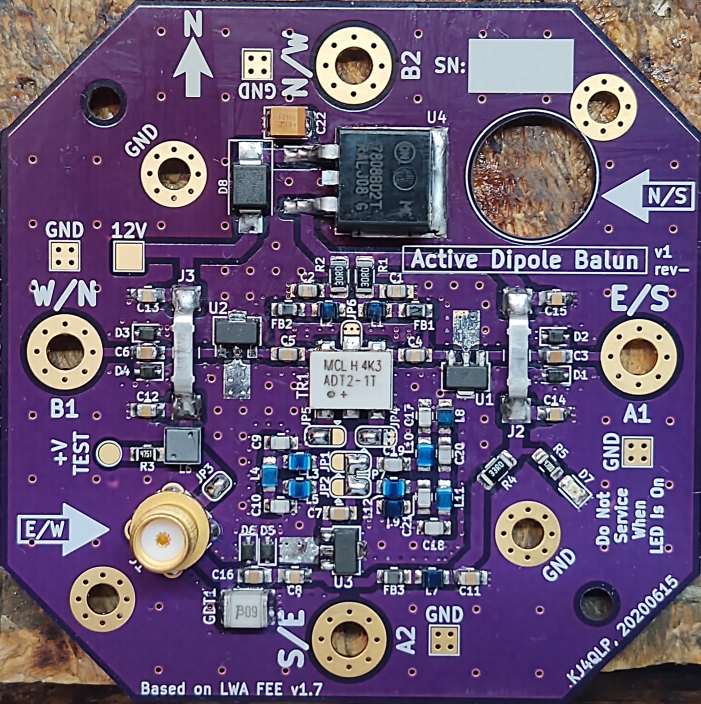
\includegraphics[width=.9\linewidth]{figures/populated_board.png}
  \end{subfigure}%
  \begin{subfigure}{.48\textwidth}
    \centering
    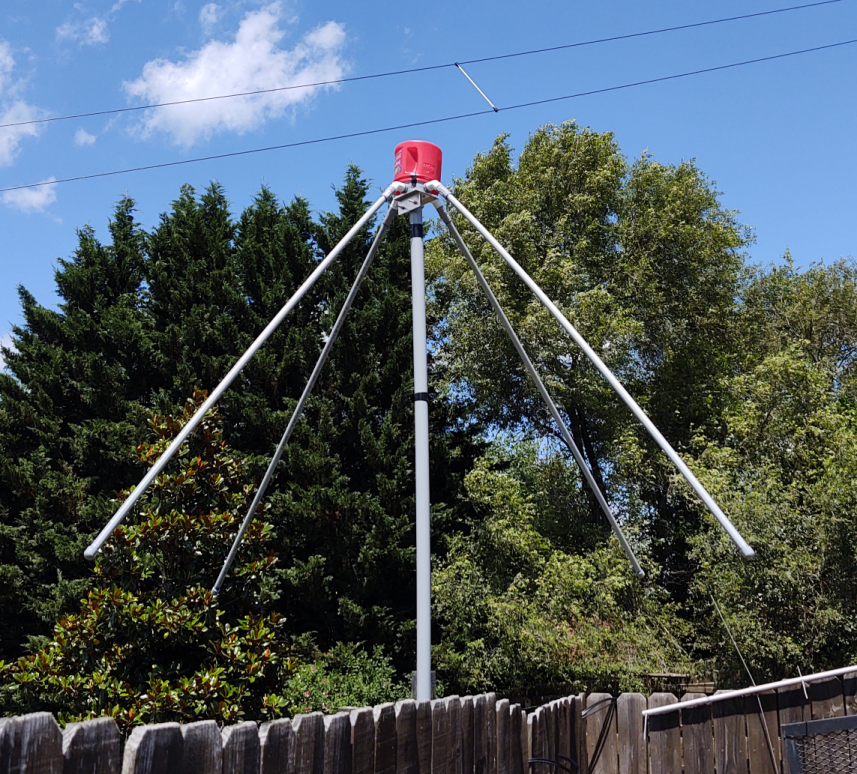
\includegraphics[width=\linewidth]{figures/crossed_inverted_v.png}
  \end{subfigure}
\end{figure}
\setcounter{figure}{0}  
\thispagestyle{title}  %This command sets both header and footer LEAVE HERE
%%--END OF TITLE PAGE SETUP-------

%%--Begin Front Matter Setup----------------
\newpage
\pagenumbering{gobble}
\pagenumbering{roman}
\fancypagestyle{fm}{
	\fancyhf{}% Clear header/footer
	\renewcommand{\footrulewidth}{1pt}
	\fancyhead[L]{\docid}
	%\fancyhead[C]{\docnum}
	\fancyhead[R]{v\docvers}
	\fancyfoot[L]{\docdate}% Left footer
	\fancyfoot[C]{\docprepcall}
	\fancyfoot[R]{\thepage}
}
\pagestyle{fm}% Set page style to plain.
\tableofcontents
%\newpage
\listoffigures
%\newpage
\listoftables
%\newpage
%%--END OF FRONT MATTER SETUP---------------

%%--Begin Subfile imports for the sections-------
\pagenumbering{gobble}
\pagenumbering{arabic}
\fancypagestyle{plain}{
	\fancyhf{}% Clear header/footer
	\fancyhead[L]{\docid}
	%\fancyhead[C]{\docnum}
	\fancyhead[R]{\docvers}
	\fancyfoot[L]{\docdate}% Left footer
	\fancyfoot[R]{\thepage / \pageref{LastPage}}% Right footer
	\fancyfoot[C]{\docprepcall}
}
\pagestyle{plain}% Set page style to plain.

%\subfile{sections/general_information}
\subfile{sections/executive_summary}
\subfile{sections/introduction}
\subfile{sections/technical_design}
\subfile{sections/schematic}
\subfile{sections/measurement}
\subfile{sections/prototype}
%%INSERT MORE SUBFILES WITH CONTENT HERE
\subfile{sections/conclusion}
%\subfile{sections/revisions}
\bibliographystyle{IEEEtran}
\bibliography{sections/references}

\end{document}
